%% vim: set tw=0 wm=0 wrap linebreak:
\title{Sample Return Challenge Proposal}
\author{
        Russel Howe\\
            \and
        Jascha Little\\
		    \and
	    Zac Lizer\\
}
\date{\today}

\documentclass[12pt]{article}
\usepackage{graphicx}
\usepackage{grffile}
\usepackage{hyperref}

\begin{document}
\maketitle

\begin{abstract}
Our robot will be awesome and stuff.
\end{abstract}

\section{Introduction}
This proposal documents our thought process leading up to the prototype design of a robot to compete in the sample return challenge \cite{rules}. The tightest constraint in the challenge is the time frame, only 6 months are alloted to design and implement a machine. We thus focus on readily available components and technologies with the goal of getting quickly to the testing phase of our design.

\paragraph{Outline}
The remainder of this article is organized as follows.
Section~\ref{Chassis} describes the locomotion and maneuvering system. Section~\ref{Manipulator} describes our approach to sample acquisition and storage. Section~\ref{Electronics} describes the power management, servo, and compute systems employed. Section~\ref{Perception} discusses our sensing systems. Section~\ref{Software} gitves a high-level overview of our software architecture.

\section{Chassis}\label{Chassis}
Jascha will discuss why an ATV chassis is exactly what we need already.

We are particularly fond of the TrailMaster MINI XRS (Figure~\ref{fig_gokart}) available here \url{http://gokartsusa.com/TrailMaster-Mini-XRS-Gokart-Buggy.aspx}.

\begin{figure}[htbp]
\centering
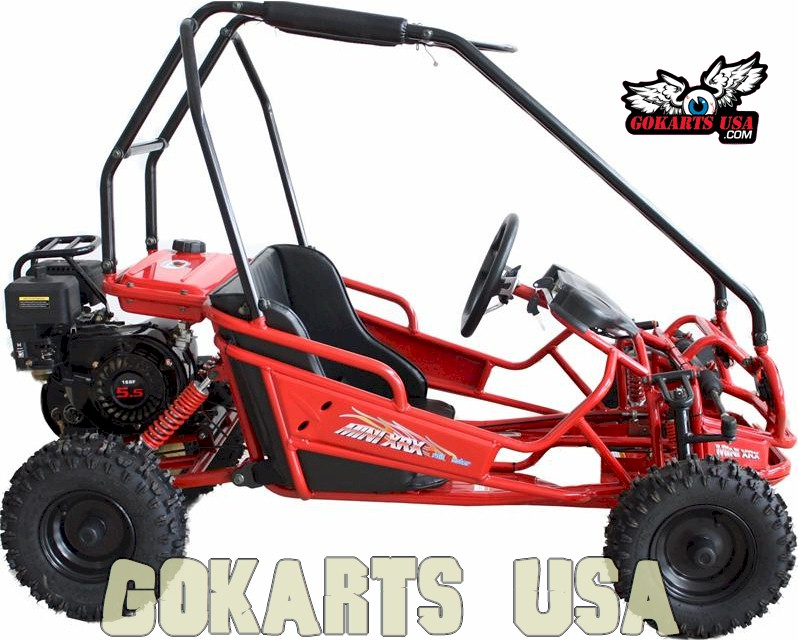
\includegraphics[width=4in]{TrailMasterMINIXRS.jpg}
\caption{The proposed vehicle chassis.}
\label{fig_gokart}
\end{figure}

The challenge rules specify an 80kg mass limit, our system allocates this as shown in Table~\ref{tab massb}.

\begin{table}[htbp]
    \begin{center}
    \begin{tabular}{lr}
        \hline
        Component & Mass (kg)\\
        \hline
        Rolling Chassis and Suspension & 25\\
        Drive Motor & 10\\
        Steering Motor & 10\\
        Batteries & 20\\
        Computers & 6\\
        Cameras & 5\\
        Manipulator & 4\\
        \hline
        \hline
        \multicolumn{1}{r}{Total} & 80\\
        \hline
    \end{tabular}
    \end{center}
    \caption{Mass Budget}
    \label{tab massb}
\end{table}

\section{Manipulator}\label{Manipulator}

Glue puck.\\

Sharp Tentacles.\\

\section{Electronics}\label{Electronics}

Battery System.\\

E-Stop design. Power On sequencing.\\

Drive motor, controller.\\

Steering servo, controller.\\

Manipulator servos, controllers.\\

Laptop Computers.\\

Assuming a mission duration of 2 hours, Table~\ref{power budget} summarizes the systems estimated power needs.

\begin{table}[htbp]
    \begin{tabular}{|l|c|c||p{4cm}|}
        \hline
        System & Demand (Watts) & Duty Cycle & Energy Requirement (Watt Hours)\\
        \hline
        Chassis Drive & 100 & 90\% & 180\\
        Steering & 25 & 90\% & 45\\
        Manipulator & 100 & 10\% & 20\\
        Compute & 200 & 100\% & 400\\
        Perception & 50 & 100\% & 100\\
        \hline
        \multicolumn{3}{|r||}{Total Energy} & 754\\
        \hline
    \end{tabular}
    \caption{2 hour Power Budget}
    \label{power budget}
\end{table}

\section{Perception}\label{Perception}
The environmental perception system consists of two stereo pairs and one high-resolution search camera. One stereo pair is aligned with the steering direction and provides the primary obstacle avoidance and navigation sensing. The other stereo pair is associated with the manipulator and provides close-in tracking and guidance for item collection. The search camera is positioned above th robot looking forward with a wide filed of view and is used by all the long-range object detectors while searching for items to be collected.

The navigational perception system consists of 4 wheel encoders for odometery, MEMS gyroscopes and precision inclinometers for attitude estimation. The attitude estimate is used to help stabilize the navigation estimate and to help align the search camera with the navigation map.

We are also exploring the possiblity of a odometery caster to provide estimates of distance traveled, it is not yet clear if this will provide sufficiently higher quality data than the wheel encoders to be worthwhile.

\section{Software}\label{Software}
Our software uses the ROS framework \url{http://www.ros.org/} to provide structure and inter-module communication. In addition, ROS has a large library of general-purpose modules which allows us to take advantage of significant expertise outside our immediate team.

\subsection{Navigation}\label{Navigation}
\begin{figure}[htbp]
\centering
\includegraphics[width=4in]{data_flow.dot.pdf}
\caption{Navigation data flow}
\label{fig_df_nav}
\end{figure}
Figure~\ref{fig_df_nav} gives an overview of the navigation system dataflow. The primary navigation utility is visual odometery as described in \cite{KKonoLSVO}. This is used to form a global feature map for large-scale navigation. The output of this system is used throughout the robot to relate measurements separated in time and space.

In addition, a local 2.5D occupancy grid is made based on obstacle detections for maneuver planning. This occupancy grid incorporates a local piece of the global data provided by satellite imagery as a prior on obstacle occupancy of a cell.

\subsection{Search}\label{Search}
\begin{figure}[htbp]
\centering
\includegraphics[width=6in]{data_flow.dot.2.pdf}
\caption{Goal Search data flow}
\label{fig_df_gs}
\end{figure}
As show in Figure~\ref{fig_df_gs}, the each goal item has its own recognizer. Several of these share large pieces of functionality, but all can operate in parallel and have slightly different tunings. For example, the Tennis Ball and Colored Sphere recognizers are identical code with different search parameters.

All recognizers intersect the detection vector with an estimate of the ground plane. This estimate is constructed from the current vehicle pose and a subset of the points detected by the navigation stereo pair.

The Goal Recognizers are allowed to be noisy and produce false positives since all their measurements are accumulated in an occupancy grid. This grid encodes exclusions around detected goal and resolves conflicts between detectors. It also includes any pre-loaded information about goal position. This map is mantained globally and effectively makes a record of already-searched areas.

\subsection{Route Planning}
\begin{figure}[htbp]
\centering
\includegraphics[width=4in]{data_flow.dot.3.pdf}
\caption{Route Planning data flow}
\label{fig_df_rp}
\end{figure}
Figure~\ref{fig_df_rp} Shows the layout of the Route Planning system. The Goal Selector uses information in the Goal Occupancy Grid to decide the next goal position in the map. It then passes this information to the Route Planner which produces a path consistent with the Obstacle Occupancy Grid and the vehicle's kinematics to arrive at the goal.

How does the Goal Selector decide where to go next? Does it consider the value of the object? Certainly includes likelihood of detection and distance from robot.

\subsection{Manipulation}\label{Manipulation}
\begin{figure}[htbp]
\centering
\includegraphics[width=4.5in]{data_flow.dot.4.pdf}
\caption{Manipulation data flow}
\label{fig_df_man}
\end{figure}
See Figure~\ref{fig_df_man}.



\subsection{Mission Execution}\label{MissionExecution}
\begin{figure}[htbp]
\centering
\includegraphics[width=6.5in]{data_flow.dot.5.pdf}
\caption{Mission Execution data flow}
\label{fig_df_exec}
\end{figure}

High level executive coordinates actions of Planners and Executors.

\bibliographystyle{abbrv}
\bibliography{main}

\end{document}

